\documentclass[a4paper,11pt] {article}
\usepackage[spanish]{babel}
%\usepackage[utf8]{inputenc}
\usepackage{caratula}
\usepackage{a4wide}
%\usepackage{graphicx}
% \usepackage{dot2texi}
% \usepackage{graphs}

\begin{document}

\titulo{Trabajo Pr\'actico Nro. 2}
\fecha{02/06/2010}
\materia{Ingenier\'ia de Software I}
\grupo{}
\integrante{Dinota, Mat\'ias}{076/07}{matiasgd@gmail.com}
\integrante{Frid, Igal Pablo}{231/07}{ipfrid@gmail.com}
\integrante{Huel, Federico Ariel}{329/07}{federico.huel@gmail.com}
\integrante{Leveroni, Luciano}{360/07}{lucianolev@gmail.com}
\integrante{Mosteiro, Agust\'in}{125/07}{agustinmosteiro@gmail.com}

\maketitle

\bigskip

\section*{Introducci\'on}

El objetivo del siguiente trabajo es realizar una segunda etapa en el modelado de un sistema para una cadena de pizzer\'ias, denominada Pizza Hack. Con este fin, se utilizar\'an t\'ecnicas de ingenier\'ia del software, a saber: Diagrama de Casos de uso, Diagramas de Actividad, Diagramas de M\'aquinas de estado (FSM) y Diagrama de modelo Conceptual. A su vez, se incluyen en el presente trabajo las decisiones tomadas durante el proceso de elaboraci\'on del mismo que llevaron a la elecci\'on y confecci\'on de los distintos diagramas que se presentar\'an a continuaci\'on. 

El sistema a modelar pretende resolver las necesidades y problemas de una cadena de pizzer\'ias t\'ipica, en la que cada uno de los locales atiende al p\'ublico a trav\'es de un mostrador, y a su vez brinda la opci\'on de sentarse a consumir los productos dentro de las mesas que posee el mismo. Adem\'as, cabe aclarar que la cadena de pizzer\'ias desea mantener el mismo men\'u en todos sus locales, por lo que un cambio en el men\'u de un local deber\'a verse reflejado en la cartilla de los restantes. Tambi\'en se debe mencionar que los locales no ofrecen servicio de delivery y, en caso de que alg\'un pedido realizado en el mostrador de un local no se pueda preparar en el mismo, por falta de stock, se ofrecer\'a la posibilidad de derivar el pedido a otro local de la cadena que pueda prepararlo.

Por medio de la aplicaci\'on de las t\'ecnicas se busca explicitar la interacci\'on de los distintos actores involucrados en la utilizaci\'on del sistema, y c\'omo se relacionan los unos con los otros. A su vez explicaremos como son las principales actividades que se realizan, es decir quienes est\'an involucrados en las mismas y c\'omo se llevan a cabo.

\section*{Presunciones}

Debido a la presencia de algunas inconsistencias encontradas entre los distintos diagramas presentes en el enunciado, se tomaron las siguientes decisiones.

\begin{itemize}
    \item Pizza Hack no brinda servicio de delivery.
    \item La m\'aquina no contempla manejo de dinero.
    \item Hay un \'unico mozo por local para atender las distintas mesas.
    \item Necesariamente debe haber un encargado, un jefe de chef (puede o no haber alg\'un otro cocinero), un mozo y un repositor de stock en cada local para su correcto funcionamiento.
    \item Los pedidos siempre pasan por el encargado para ingresarse en el sistema.
    \item Cuando un pedido se realiza al mozo en una mesa, el mismo le pasa el pedido al encargado para que el mismo lo ingrese en el sistema.
    \item El operador solo se encarga de dar de alta a un nuevo local, no es un empleado del mismo.
		\item Cuando un local tiene el turno para realizar una operaci\'on que requiera comunicaci\'on con otros locales, el turno no se puede terminar en el medio de la operaci\'on.
\end{itemize}

\section*{Discusi\'on}

En primera instancia, se opt\'o por realizar un diagrama conceptual a modo de conocer los distintos conceptos involucrados en el sistema. Adem\'as, al comenzar con la elaboraci\'on del mismo se pudo reconocer atributos de los objetos junto con las formas de relacionarse entre s\'i con el objetivo de familiarizarse con las partes que lo conforman. A continuaci\'on se muestra lo realizado:

\begin{center}
 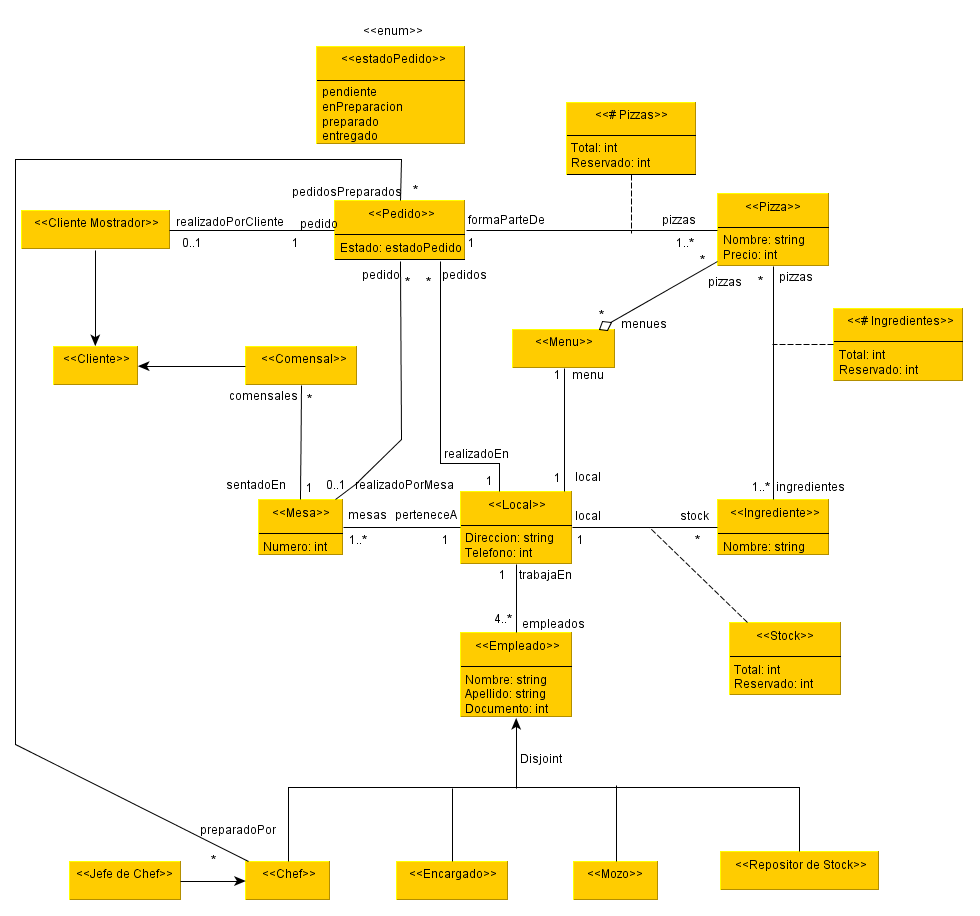
\includegraphics[width=1\textwidth]{Diagramas/DiagramaConceptual.png}
\end{center}

\subsection*{Ocl}

\textbf{Context Local}

\begin{itemize}
	\item Def: Todos los locales tienen un men\'u con mismas pizzas.
	
				$inv: Local.AllInstances()\rightarrow forAll(l | l.menu.pizzas == self.menu.pizzas);$
				
	\item	Def: Hay un repositor, un mozo, un encargado y un jefe de chef por local.
	
	$inv: self.empleados\rightarrow select(e | e.isTypeOf(Repositor de Stock))\rightarrow size() == 1 $ and $ \\
	self.empleados\rightarrow select(e | e.isTypeOf(Mozo))\rightarrow size() == 1 $ and $	\\
	self.empleados\rightarrow select(e | e.isTypeOf(Encargado))\rightarrow size() == 1 $ and $	\\
	self.empleados\rightarrow select(e | e.isTypeOf(Jefe de Chef))\rightarrow size() == 1;$	\\
	
	\item	Def: Todos los pedidos de un local son preparados por chefs del mismo local.
	
	$inv: self.pedidos\rightarrow collect(preparadoPor)\rightarrow forAll(c | self.empleados \rightarrow exists(e | e.isTypeOf(chef) $ and $e == c));$
	
	\item	Def: Todos los pedidos de un local que sean realizados por una mesa son realizados por mesas del local.
	
	$inv: self.pedidos\rightarrow collect(realizadoPorMesa)\rightarrow forAll(m | self.mesas\rightarrow exists(m' | m' = m));$
	
\end{itemize}

\textbf{Context Stock}

\begin{itemize}
	\item Def: Cada ingrediente posee un stock total mayor al reservado para realizar pizzas.
	
	$inv: self.total >= self.reservados;$
\end{itemize}

\textbf{Context Pizza}

\begin{itemize}
	\item Def: Si dos pizzas son iguales tienen la misma cantidad de cada uno de sus ingredientes.
	
	$inv: Pizzas.AllInstances()\rightarrow forAll(p1 p2 | p1 == p2 $ implies $ p1.\#ingredientes.cantidad == p2.\#ingredientes.cantidad);$
\end{itemize}

\textbf{Context Pedido}

\begin{itemize}
	\item Def: Los pedidos son hechos por un cliente en el mostrador o por una mesa.
	
	$inv: self.realizadoPorCliente\rightarrow size() + self.realizadoPorMesa\rightarrow size() == 1;$
	
	\item Def: Si el pedido no esta pendiente hay al menos un chef involucrado en su preparaci�n.
	
	$inv: self.estadoPedido \neq pendiente$ implies $self.preparadoPor\rightarrow size() > 0;$
\end{itemize}


\bigskip

Una vez fijados los conceptos, se procedi\'o a desarrollar un diagrama de casos de uso ya que, en primera instancia, se pueden desprender interacciones y agentes f\'acilmente del diagrama de contexto provisto. Sin embargo, al observar los escenarios se not\'o que los agentes presentes en el sistema realizaban distintas actividades no contempladas o de manera distinta a lo expuesto en el diagrama de contexto. Luego de una discusi\'on extensa sobre que tener en cuenta en cada diagrama, el grupo decidi\'o en dar m\'as relevancia a los escenarios presentados ya que resultaban m\'as coherentes a la idea general del sistema.

A continuaci\'on se presenta el diagrama de casos de uso realizado junto con las descripciones asociadas:

\begin{center}
 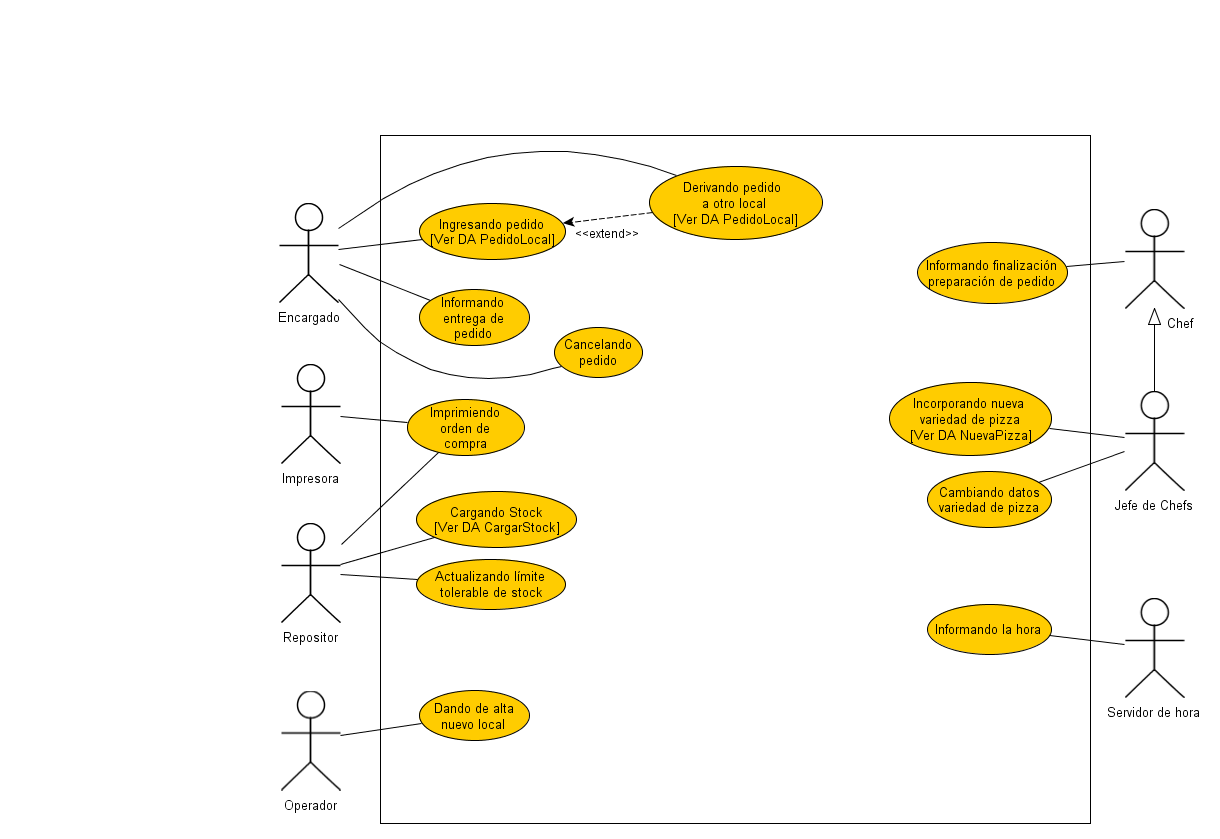
\includegraphics[width=1\textwidth]{Diagramas/CasosDeUso.png}
\end{center}

\textbf{Detalle Casos de uso}

\begin{center}
	\begin{tabular}{ | p{6.5cm} | p{6.5cm} | }
		\hline
			\multicolumn{2}{|l|}{\textbf{Caso de Uso:} Ingresando pedido} \\
		\hline
			\multicolumn{2}{|l|}{\textbf{Actores:} Encargado} \\
		\hline
			\multicolumn{2}{|l|}{\textbf{Pre:} True} \\
		\hline
			\multicolumn{2}{|l|}{\textbf{Post:} Si el pedido es realizable, el pedido es ingresado} \\
		\hline
			\textbf{Caso Normal} & \textbf{Caso Alternativo}	\\
		\hline
		1. El encargado ingresa al sistema cada pizza que el cliente ordena. &	\\
		\hline
		2. El sistema le informa al encargado si el pedido se puede realizar. &	\\
		\hline
		2.1. En caso afirmativo, se reservan los ingredientes necesarios para preparar el pedido, luego ir al fin de caso de uso. &	\\
		\hline
		2.2. Si no se puede realizar, el sistema busca si se puede realizar en otro local. &	\\
		\hline
		3.1 Si se puede realizar en otro local, EXTIENDE CASO DE USO "`Derivando pedido a otro local"' &	\\
		\hline
		3.2 Si no se puede, se le informa de esto al encargado y el mismo le comunica al cliente que no puede realizar la compra. &	\\
		\hline
		4. Fin de caso de uso. &	\\
		\hline
	\end{tabular}
\end{center}

\begin{center}
	\begin{tabular}{ | p{6.5cm} | p{6.5cm} | }
		\hline
			\multicolumn{2}{|l|}{\textbf{Caso de Uso:} Cancelando pedido} \\
		\hline
			\multicolumn{2}{|l|}{\textbf{Actores:} Encargado} \\
		\hline
			\multicolumn{2}{|l|}{\textbf{Pre:} El pedido debe estar pendiente} \\
		\hline
			\multicolumn{2}{|l|}{\textbf{Post:} El pedido es cancelado} \\
		\hline
		\textbf{Caso Normal} & \textbf{Caso Alternativo}	\\
		\hline
		1. El encargado ingresa al sistema el pedido que desea cancelar. &	\\
		\hline
		2. El sistema le quita la reserva a los ingredientes que se hab\'ian reservado para ese pedido. &	\\
		\hline
		3. El sistema cancela el pedido y lo quita de la cola de pedidos pendientes. &	\\
		\hline
		4. Fin de caso de uso. &	\\
		\hline
	\end{tabular}
\end{center}

\begin{center}
	\begin{tabular}{ | p{6.5cm} | p{6.5cm} | }
		\hline
			\multicolumn{2}{|l|}{\textbf{Caso de Uso:} Derivando pedido a otro local} \\
		\hline
			\multicolumn{2}{|l|}{\textbf{Actores:} Encargado} \\
		\hline
			\multicolumn{2}{|l|}{\textbf{Pre:} Se ingres\'o un pedido que puede ser derivado.} \\
		\hline
			\multicolumn{2}{|l|}{\textbf{Post:} Pedido derivado.} \\
		\hline
		\textbf{Caso Normal} & \textbf{Caso Alternativo}	\\
		\hline
		1. El sistema le informa al encargado cuales son los locales que tienen stock para tomar el pedido. [Ver FSM B\'usqueda locales para derivar] &	\\
		\hline
		2.1. Si el cliente est� conforme con alguna de las opciones, el encargado selecciona dicha opci\'on. &	\\
		\hline
		2.2. En caso contrario el pedido no se deriva. &	\\
		\hline
		3. Si se acept\'o la derivaci\'on, se reservan los ingredientes necesarios para preparar el pedido. &	\\
		\hline
		4. Fin de caso de uso. &	\\
		\hline
	\end{tabular}
\end{center}

\begin{center}
	\begin{tabular}{ | p{6.5cm} | p{6.5cm} | }
		\hline
			\multicolumn{2}{|l|}{\textbf{Caso de Uso:} Informando entrega de pedido} \\
		\hline
			\multicolumn{2}{|l|}{\textbf{Actores:} Encargado} \\
		\hline
			\multicolumn{2}{|l|}{\textbf{Pre:} Hay un pedido listo para entregar} \\
		\hline
			\multicolumn{2}{|l|}{\textbf{Post:} Informe de entrega realizado} \\
		\hline
		\textbf{Caso Normal} & \textbf{Caso Alternativo}	\\
		\hline
		1. El encargado le indica al sistema que un pedido pendiente de entrega ha sido entregado al cliente. &	\\
		\hline
		2. Fin de caso de uso. &	\\
		\hline
	\end{tabular}
\end{center}

\begin{center}
	\begin{tabular}{ | p{6.5cm} | p{6.5cm} | }
		\hline
			\multicolumn{2}{|l|}{\textbf{Caso de Uso:} Imprimiendo orden de compra} \\
		\hline
			\multicolumn{2}{|l|}{\textbf{Actores:} Repositor, Impresora} \\
		\hline
			\multicolumn{2}{|l|}{\textbf{Pre:} True} \\
		\hline
			\multicolumn{2}{|l|}{\textbf{Post:} Orden de compra impresa} \\
		\hline
		\textbf{Caso Normal} & \textbf{Caso Alternativo}	\\
		\hline
		1. Se realiza orden de compra al sistema por falta de stock. &	\\
		\hline
		2. El sistema le env\'ia a la impresora la \'orden a imprimir. &	\\
		\hline
		3. Una vez impresa la \'orden, el repositor la retira de la impresora. & 3. La impresora no dispone de los insumos necesarios para realizar la impresi\'on.	\\
		\hline
		4. Fin de caso de uso. & 4. Fin de caso de uso.	\\
		\hline
	\end{tabular}
\end{center}

\begin{center}
	\begin{tabular}{ | p{6.5cm} | p{6.5cm} | }
		\hline
			\multicolumn{2}{|l|}{\textbf{Caso de Uso:} Cargando Stock} \\
		\hline
			\multicolumn{2}{|l|}{\textbf{Actores:} Repositor} \\
		\hline
			\multicolumn{2}{|l|}{\textbf{Pre:} True} \\
		\hline
			\multicolumn{2}{|l|}{\textbf{Post:} Stock cargado.} \\
		\hline
		\textbf{Caso Normal} & \textbf{Caso Alternativo}	\\
		\hline
		1. El repositor va ingresando al sistema cada ingrediente que fue repuesto con su correspondiente cantidad. &	\\
		\hline
		2. Se repite el paso 1 hasta que el respositor haya terminado de cargar todos los ingrediente repuestos. &	\\
		\hline
		3. Fin de caso de uso. &	\\
		\hline
	\end{tabular}
\end{center}

\begin{center}
	\begin{tabular}{ | p{6.5cm} | p{6.5cm} | }
		\hline
			\multicolumn{2}{|l|}{\textbf{Caso de Uso:} Actualizando l\'imite tolerable de stock.} \\
		\hline
			\multicolumn{2}{|l|}{\textbf{Actores:} Repositor} \\
		\hline
			\multicolumn{2}{|l|}{\textbf{Pre:} True} \\
		\hline
			\multicolumn{2}{|l|}{\textbf{Post:} Stock cargado.} \\
		\hline
		\textbf{Caso Normal} & \textbf{Caso Alternativo}	\\
		\hline
		1. El repositor selecciona el ingrediente del cual quiere actualizar el limite tolerable. &	\\
		\hline
		2. Se ingresa un nuevo valor y se aplican los cambios. & 2. El valor ingresado es inv�lido y el sistema le informa al repositor que ingrese otro valor.	\\
		\hline
		3. Fin de caso de uso. & 3. Fin de caso de uso.	\\
		\hline
	\end{tabular}
\end{center}

\begin{center}
	\begin{tabular}{ | p{6.5cm} | p{6.5cm} | }
		\hline
			\multicolumn{2}{|l|}{\textbf{Caso de Uso:} Informando finalizaci\'on preparaci\'on de pedido.} \\
		\hline
			\multicolumn{2}{|l|}{\textbf{Actores:} Chef} \\
		\hline
			\multicolumn{2}{|l|}{\textbf{Pre:} True} \\
		\hline
			\multicolumn{2}{|l|}{\textbf{Post:} El pedido figura como preparado.} \\
		\hline
		\textbf{Caso Normal} & \textbf{Caso Alternativo}	\\
		\hline
		1. El chef selecciona el pedido que termin\'o y lo marca como terminado en el sistema. &	\\
		\hline
		2. El sistema actualiza el estado del pedido, pasando dicho pedido a pendiente de entrega. &	\\
		\hline
		3. Se descuenta el stock utilizado en el pedido. &	\\
		\hline
		4. Fin de caso de uso. &	\\
		\hline
	\end{tabular}
\end{center}

\begin{center}
	\begin{tabular}{ | p{6.5cm} | p{6.5cm} | }
		\hline
			\multicolumn{2}{|l|}{\textbf{Caso de Uso:} Incorporando nueva variedad de pizza} \\
		\hline
			\multicolumn{2}{|l|}{\textbf{Actores:} Jefe de chefs} \\
		\hline
			\multicolumn{2}{|l|}{\textbf{Pre:} True} \\
		\hline
			\multicolumn{2}{|l|}{\textbf{Post:} Nueva variedad de pizza cargada} \\
		\hline
		\textbf{Caso Normal} & \textbf{Caso Alternativo}	\\
		\hline
		1. El jefe de chefs ingresa el nombre de la nueva pizza a ingresar. & 1.1 La pizza ya existe. Ir a fin de caso de uso.	\\
		\hline
		2. El jefe de chefs ingresa un ingrediente y su cantidad. &	\\
		\hline
		3. Se repite el paso 2 hasta que no queden ingredientes por agregar. &	\\
		\hline
		4. Se ingresa el precio de pizza. &	\\
		\hline
		5. El sistema registra la nueva variedad de pizza, actualizando el men\'u en todos los locales [Ver FSM ActualizacionMenu]. &	\\
		\hline
		6. Fin de caso de uso. & 6. Fin de caso de uso.	\\
		\hline
	\end{tabular}
\end{center}

\begin{center}
	\begin{tabular}{ | p{6.5cm} | p{6.5cm} | }
		\hline
			\multicolumn{2}{|l|}{\textbf{Caso de Uso:} Cambiando datos variedad de pizza} \\
		\hline
			\multicolumn{2}{|l|}{\textbf{Actores:} Jefe de chefs} \\
		\hline
			\multicolumn{2}{|l|}{\textbf{Pre:} True} \\
		\hline
			\multicolumn{2}{|l|}{\textbf{Post:} Datos de la variedad de pizza modificados.} \\
		\hline
		\textbf{Caso Normal} & \textbf{Caso Alternativo}	\\
		\hline
		1. El jefe de chefs selecciona en el sistema la variedad de pizza que desea modificar. & 	\\
		\hline
		2. El jefe de chefs modifica los datos de cualquiera de los ingredientes y su cantidad.  &	\\
		\hline
		3. Se repite el paso 2 hasta que el jefe de chefs termina de modificar todos los ingredientes que desee cambiar. &	\\
		\hline
		4. El sistema registra los cambios en la variedad de pizza y modifica el men\'u en todos los locales [Ver FSM ActualizacionMenu].  &	\\
		\hline
		5. Fin de caso de uso. &	\\
		\hline
	\end{tabular}
\end{center}

\begin{center}
	\begin{tabular}{ | p{6.5cm} | p{6.5cm} | }
		\hline
			\multicolumn{2}{|l|}{\textbf{Caso de Uso:} Informando la hora} \\
		\hline
			\multicolumn{2}{|l|}{\textbf{Actores:} Servidor de hora.} \\
		\hline
			\multicolumn{2}{|l|}{\textbf{Pre:} True} \\
		\hline
			\multicolumn{2}{|l|}{\textbf{Post:} El sistema conoce la hora del servidor de hora.} \\
		\hline
		\textbf{Caso Normal} & \textbf{Caso Alternativo}	\\
		\hline
		1. El sistema solicita la hora al servidor de hora. & 1. El servidor de hora no se encuentra disponible. Ir a fin de caso de uso.	\\
		\hline
		2. El sistema recibe la respuesta del servidor de hora. &	\\
		\hline
		3. Fin de caso de uso. & 3. Fin de caso de uso.	\\
		\hline
	\end{tabular}
\end{center}

\begin{center}
	\begin{tabular}{ | p{6.5cm} | p{6.5cm} | }
		\hline
			\multicolumn{2}{|l|}{\textbf{Caso de Uso:} Dando de alta nuevo local} \\
		\hline
			\multicolumn{2}{|l|}{\textbf{Actores:} Operador} \\
		\hline
			\multicolumn{2}{|l|}{\textbf{Pre:} True} \\
		\hline
			\multicolumn{2}{|l|}{\textbf{Post:} Local registrado en el sistema} \\
		\hline
		\textbf{Caso Normal} & \textbf{Caso Alternativo}	\\
		\hline
		1. El operador registra los datos del local en el sistema. & 1.1. El local ya se encuentra registrado en el sistema. Ir a fin de caso de uso.	\\
		\hline
		2. El sistema crea un men\'u vac\'io para el local registrado. &	\\
		\hline
		3. Si ya existe un local registrado, el sistema obtiene el men\'u de cualquiera de los locales registrados y se lo asigna al nuevo local &	\\
		\hline
		4. El sistema notifica a los dem�s locales el nuevo local registrado. &	\\
		\hline
		5. Fin de caso de uso &	5. Fin de caso de uso \\
		\hline
	\end{tabular}
\end{center}

Luego de tener en claro el rol de los diferentes actores en el sistema, se empez\'o a analizar que casos de uso resultaban interesantes describir m\'as en detalle. En primer lugar, se opt\'o por observar el caso de uso \textit{Ingresando pedido} ya que resulta ser una de las tareas principales del sistema. Luego de una breve discusi\'on, se decidi\'o por realizar un diagrama de actividad ya que es el que mejor describe lo que sucede globalmente en los casos donde interviene dicha interacci\'on con el sistema. Al comenzar con dicho diagrama, se not\'o que hab\'ia dos escenarios ligeramente distintos al momento de ingresar un nuevo pedido. Por un lado, el cliente podr\'ia interactuar directamente con el encargado en caso de que se trate de una persona que va a realizar un pedido para llevar o bien ser\'a el mozo quien le comunique los pedidos al encargado si se trata de un simple comensal sentado en una mesa (Ver \textit{Cliente Mostrador} y \textit{Comensal} en el Diagrama Conceptual). Por este motivo, se realizaron los siguientes dos diagramas de actividad para mostrar ambas situaciones:

\begin{center}
 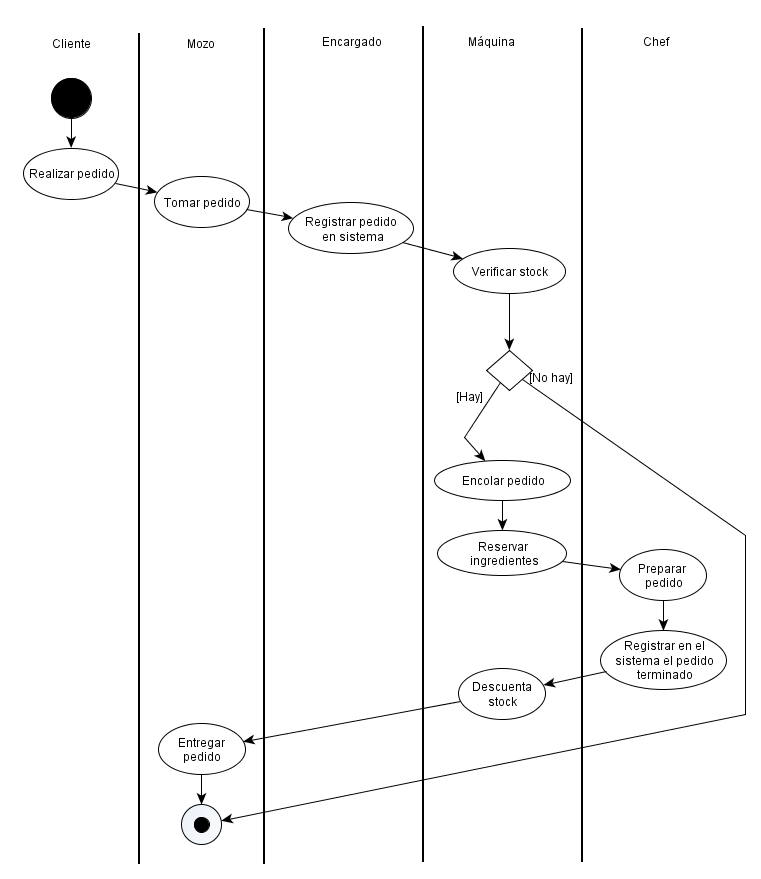
\includegraphics[width=0.7\textwidth]{Diagramas/DiagramaActividadPedidoLocalMesa.png}
\end{center}

\begin{center}
 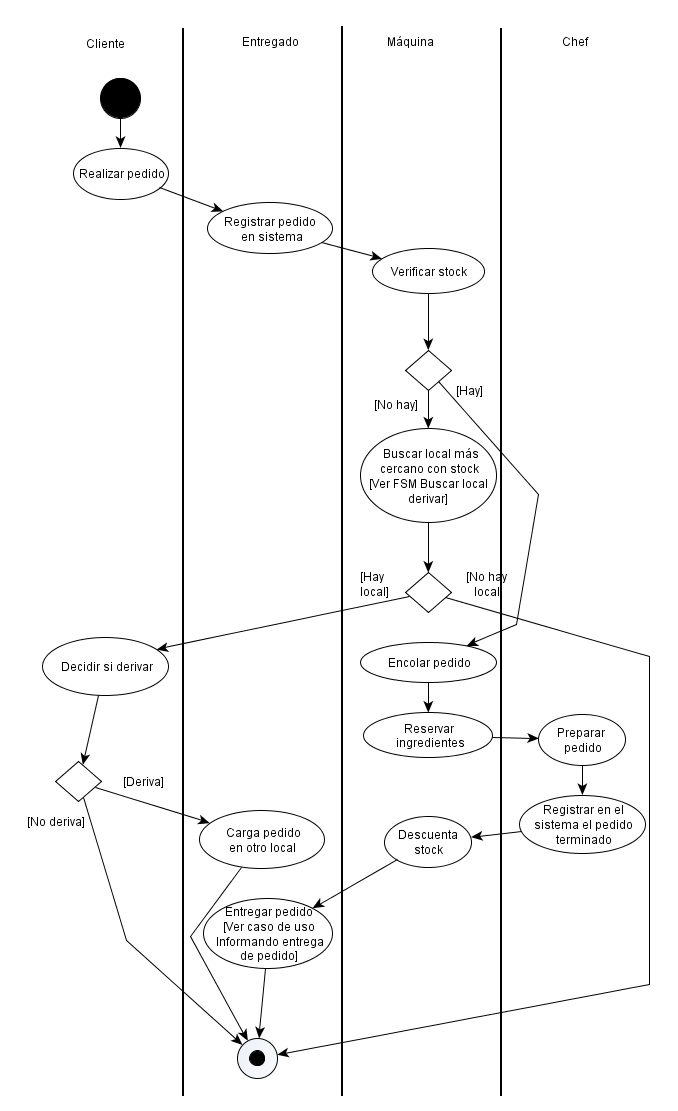
\includegraphics[width=0.7\textwidth]{Diagramas/DiagramaActividadPedidoLocal.png}
\end{center}

Como se puede observar, el diagrama contiene a las actividades referenciadas en los casos de uso \textit{Derivando pedido a otro local} y \textit{Informando entrega de pedido}. La raz\'on de esto es que ambas actividades se encuentran intimamente relacionadas con lo que sucede al ingresar un pedido. Sin embargo, se vi\'o que resultaba interesante presentar tambi\'en un diagrama de actividad que describiera lo que sucede al recibir una derivaci\'on de parte de otro local ya que los diagramas anteriores no explicitaban este hecho.

\begin{center}
 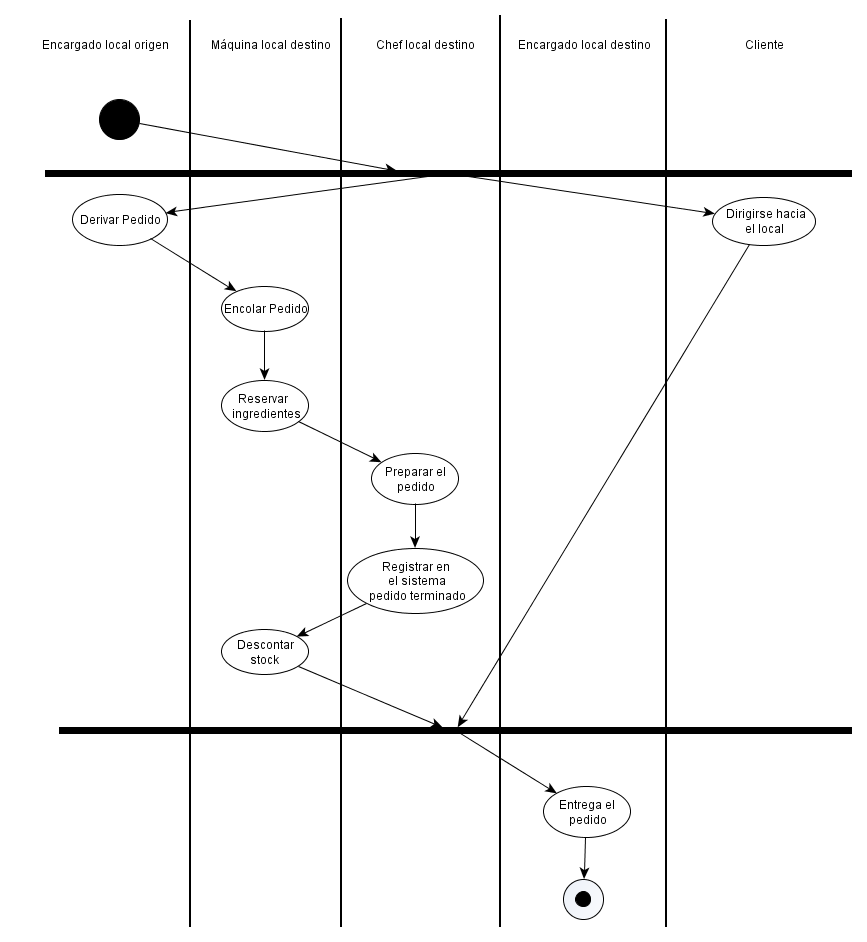
\includegraphics[width=0.7\textwidth]{Diagramas/DiagramaActividadPedidoExterno.png}
\end{center}

En los diagramas presentados se puede notar referencias a una M\'aquina de Estado llamada \textit{Buscar local derivar}. Este diagrama tiene como objetivo mostrar el comportamiento en detalle de la b\'usqueda de los locales en donde se pueda derivar un pedido no realizable localmente. Al tratarse de una operaci\'on sincronizada realizada exclusivamente por las m\'aquinas de los locales, pareci\'o oportuno utilizar este tipo de esquema como se muestra a continuaci\'on:

\begin{center}
 \textit{FSM: M\'aquina Derivadora}
 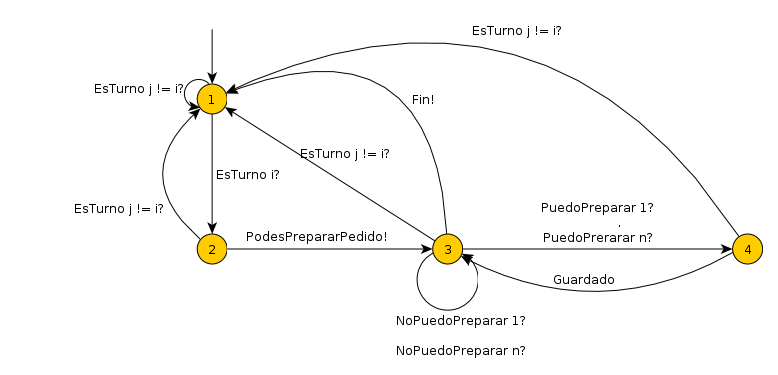
\includegraphics[width=0.7\textwidth]{Diagramas/FSMPrepararPedido.png}
\end{center}
\begin{center}
 \textit{FSM: M\'aquina$_{i}$}
 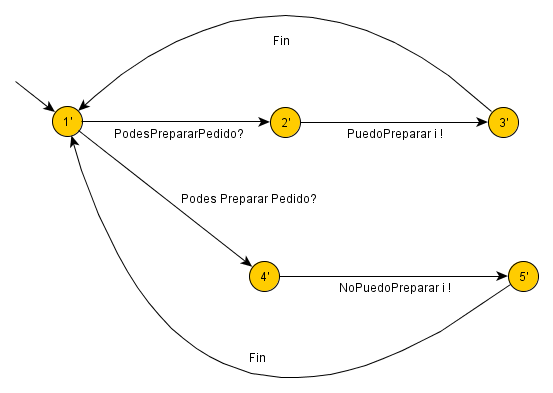
\includegraphics[width=0.7\textwidth]{Diagramas/FSMPrepararPedidoi.png}
\end{center}

Continuando con el diagrama de casos de uso, los siguientes casos analizados fueron los relativos al Jefe de Chef: \textit{Incorporando nueva variedad de pizza} y \textit{Cambiando datos variedad de pizza}. Al igual que antes, para profundizar lo vinculado a estos casos se decidi\'o hacer un diagrama de actividad que muestre que sucede al querer incorporar una nueva variedad de pizza. No se crey\'o necesario mostrar el caso en el que se cambian los datos porque resulta muy similar caso a continuaci\'on elaborado:

\begin{center}
 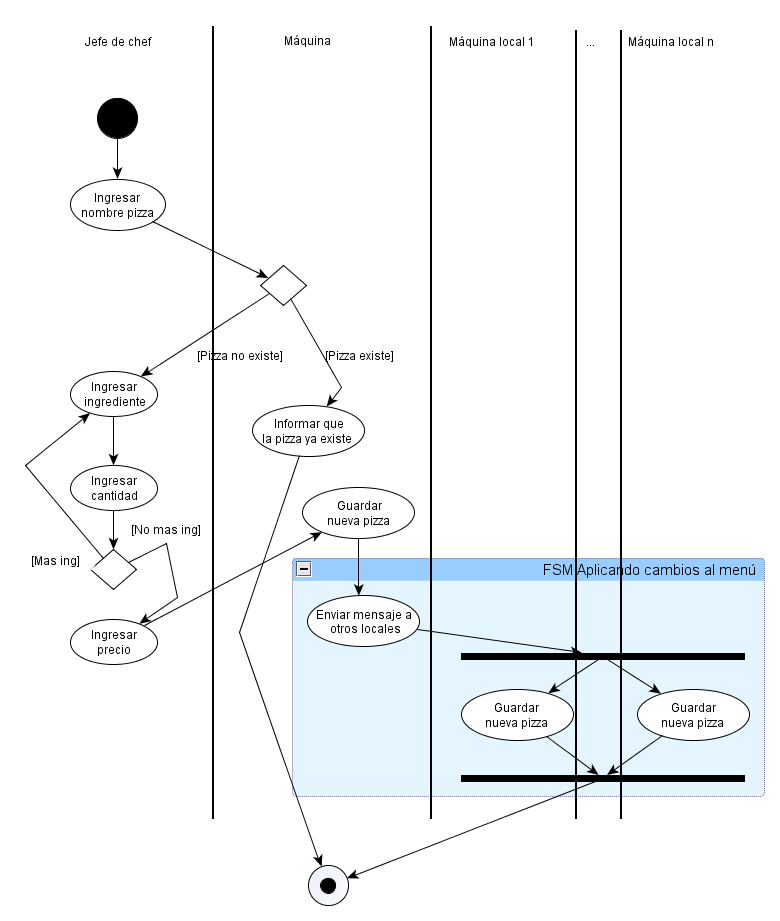
\includegraphics[width=0.7\textwidth]{Diagramas/DiagramaActividadNuevaPizza.png}
\end{center}

Esta actividad tiene la particularidad de involucrar a la m\'aquina de todos los locales del sistema por lo cual, tal como se ve en la figura, se procedi\'o a confeccionar una M\'aquina de Estado. Como el caso anterior, de esta manera se puede reflejar como funciona operacionalmente el proceso de comunicacion y sincronizacion al momento de querer informar al resto de los locales de los cambios efectuados.

\begin{center}
 \textit{FSM: M\'aquina Actualizadora}
 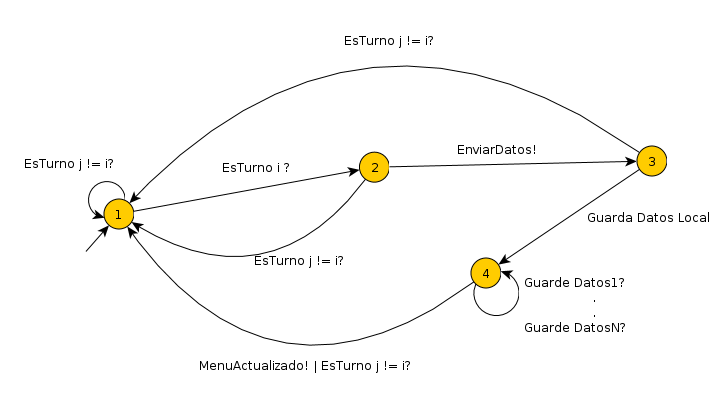
\includegraphics[width=0.7\textwidth]{Diagramas/FSMActualizacionActualizadora.png}
\end{center}
\begin{center}
 \textit{FSM: M\'aquina$_{i}$}
 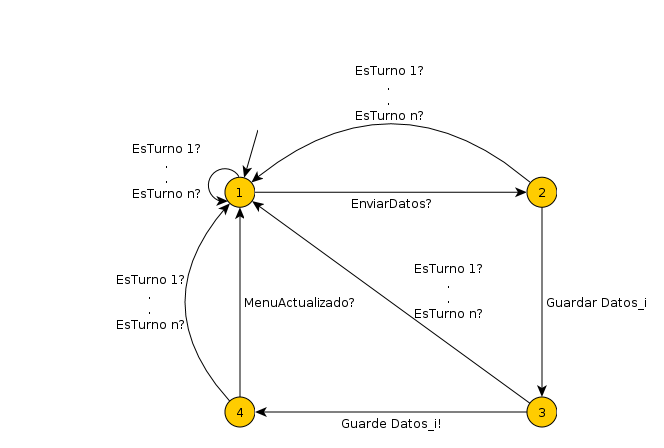
\includegraphics[width=0.7\textwidth]{Diagramas/FSMActualizacionMaquinai.png}
\end{center}

Retornando nuevamente al diagrama principal de casos de uso, por \'ultimo interes\'o incluir un diagrama que muestre que ocurre al tener que realizar una reposici\'on de stock, de manera de mostrar interacciones no observables en el caso de uso en cuesti\'on. A continuaci\'on, se muestra este diagrama:

\begin{center}
 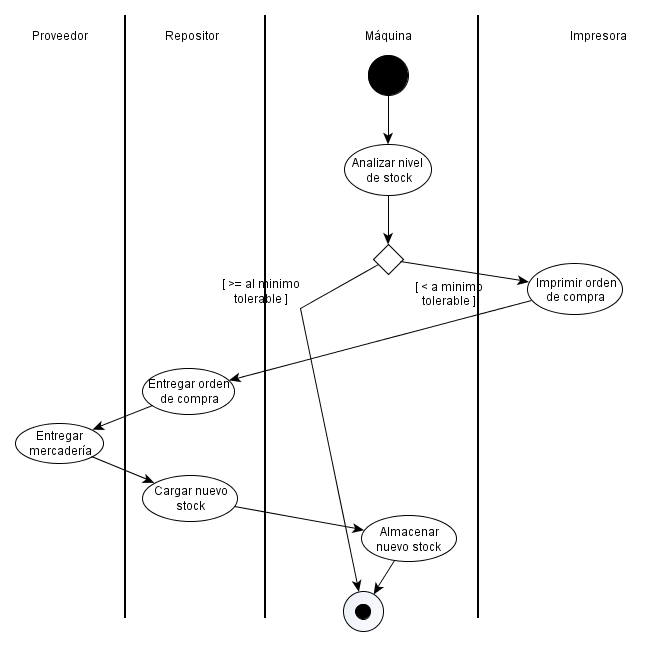
\includegraphics[width=0.7\textwidth]{Diagramas/DiagramaActividadReponerStock.png}
\end{center}

\section*{Conclusiones Generales}

A la hora de encarar el trabajo pr\'actico se presentaron varios caminos posibles por los cuales
comenzar con el modelado requerido. Pudimos haber comenzado realizando el diagrama de
casos de uso o el diagrama de modelo conceptual, ya que el resto de los diagramas, al ser tan espec\'ificos, podr\'ian surgir a partir de los diagramas mencionados. Luego de una discusi\'on se opt\'o por realizar primero el diagrama de modelo conceptual ya que nos pareci\'o m\'as conveniente tener primero una visi\'on global de los conceptos que forman parte del sistema, para luego tener en claro cu\'ales ser\'ian las interacciones entre los diferentes actores del sistema.

Una vez realizado el modelo conceptual se procedi\'o al desarrollo del diagrama de casos de uso, el cual era el otro diagrama general que deb\'iamos realizar.

A partir del mismo salieron a la luz las actividades principales del sistema, las cuales fueron expllicadas en los diagramas de actividad. Hicimos primero los diagramas de actividad antes que las FSM ya que nos parec\'ia muy complicado realizar esta \'ultima tarea porque no cont\'abamos con los conocimientos necesarios en ese momento. Luego de realizar consultas a los docentes, estuvimos en condiciones de realizar los diagramas de FSM que nos parecieron pertinentes. El criterio utilizado fue modelar mediante FSM toda funcionalidad que requiera cierta sincronizaci\'on entre las distintas m\'aquinas.

Entre los principales problemas que se presentaron estuvo el hecho de que el material brindado no era del todo consistente, por lo que tuvimos que tomar varias decisiones, lo cual consumi\'o bastante tiempo hasta que llegamos a un esquema libre de contradicciones. 

Durante la realizaci\'on del diagrama de modelo conceptual, surgieron varias discusiones sobr\'e cu\'ales eran los aspectos a tener en cuenta. Esto desencaden\'o en la necesidad de rehacer el diagrama por completo una vez que estaba casi finalizado. La causa principal del conflicto fue el hecho de que aparecieran mesas y mozos (los cuales no estaban en el trabajo pr\'actico anterior) que no sab\'iamos bien como tratar. Luego de una larga discusi\'on decidimos que en cada local haya solo un mozo para atender todas las mesas (ver presunciones).

Como conclusi\'on final del trabajo pudimos observar que al tener realizados todos los diagramas presentados, tuvimos una visi\'on muy amplia y completa de todas las funcionalidades del sistema, como asi tambi\'en de la interacci\'on entre todos los involucrados en el mismo. Adem\'as pudimos conocer con cierta profundidad el detalle de cada actividad y responsabilidad de cada individuo que forma parte del sistema. Sin conocer todos estos datos, no estar\'iamos en condiciones de comenzar con la etapa de dise\~{n}o del software ya que cualquier interpretaci\'on incorrecta de alguna funcionalidad representar\'ia un costo muy alto en un futuro. Es por esto que consideramos muy importante realizar esta etapa en el desarrollo de software.

\end{document}